\documentclass{article}
\usepackage[
    margin=0pt,
    paperwidth=11.5cm,
    paperheight=4.35cm
]{geometry}
\usepackage{import}
\subimport{../../}{preamble}
\subimport{../../}{tikz-config}

\begin{document}

\begin{figure}[t!]
\centering
\begin{subfigure}[t]{.49\textwidth}
\caption{Balanced graph}
\vspace{1em}
\centering
\begin{tikzpicture}[
    node distance=1cm,
    vnode/.style = {vertex, minimum size=1.2em}
]
    \node[vnode] (v1) {};
    \node[vnode, above left of=v1] (v2) {};
    \node[vnode, below left of=v1] (v3) {};
    \begin{pgfonlayer}{background}
        \node[draw, circle, fit=(v1)(v2)(v3), fill=green!20!yellow!20] {};
    \end{pgfonlayer}

    \path[draw, edge]
        (v1) edge[plus] (v2)
        (v2) edge[plus] (v3)
        (v3) edge[plus] (v1);

    \node[vnode, right of=v1, node distance=2cm] (v4) {};
    \node[vnode, above right of=v4] (v5) {};
    \node[vnode, below right of=v4] (v6) {};
    \begin{pgfonlayer}{background}
        \node[draw, circle, fit=(v4)(v5)(v6), fill=brown!10] {};
    \end{pgfonlayer}

    \path[draw, edge]
        (v4) edge[plus] (v5)
        (v4) edge[plus] (v6)
        (v5) edge[plus] (v6);

    \path[draw, edge]
        (v1) edge[minus] (v4);

\end{tikzpicture}
\end{subfigure}
\hfill
\begin{subfigure}[t]{.49\textwidth}
\caption{Max. unbalanced graph}
\vspace{1em}
\centering
\begin{tikzpicture}[
    node distance=1cm,
    vnode/.style = {vertex, minimum size=1.2em}
]
    \node[vnode] (v1) {};
    \node[vnode, above left of=v1] (v2) {};
    \node[vnode, below left of=v1] (v3) {};
    \begin{pgfonlayer}{background}
        \node[draw, circle, fit=(v1)(v2)(v3), fill=green!20!yellow!20] {};
    \end{pgfonlayer}

    \path[draw, edge]
        (v1) edge[minus] (v2)
        (v2) edge[minus] (v3)
        (v3) edge[minus] (v1);

    \node[vnode, right of=v1, node distance=2cm] (v4) {};
    \node[vnode, above right of=v4] (v5) {};
    \node[vnode, below right of=v4] (v6) {};
    \begin{pgfonlayer}{background}
        \node[draw, circle, fit=(v4)(v5)(v6), fill=brown!10] {};
    \end{pgfonlayer}

    \path[draw, edge]
        (v4) edge[minus] (v5)
        (v4) edge[minus] (v6)
        (v5) edge[minus] (v6);

    \path[draw, edge]
        (v1) edge[plus] (v4);
        
\end{tikzpicture}
\end{subfigure}

\vspace{.5em}
\begin{subfigure}[t]{\textwidth}
\centering
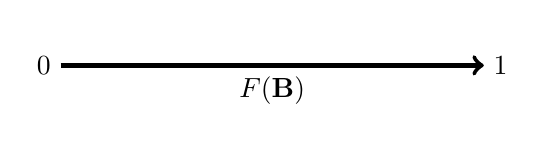
\begin{tikzpicture}
    \node[label] (zero) {$0$}; 
    \node[label, right of=zero, node distance=5.8cm] (one) {$1$};
    \draw[->, ultra thick]
        (zero)--node[label, below]{$F(\mathbf{B})$}(one);
\end{tikzpicture}
\end{subfigure}
\end{figure}

\end{document}
